\subsection{Análisis de SW}

\subsubsection{Firmware}

De forma general, el firmware desarrollado genera el comportamiento deseado cuando se carga en el Arduino UNO. Esto se puede afirmar con base en que la intensidad luminosa de la bombilla cambia correctamente en función de la posición de una mano ante la 


Este consta de varias secciones de interés: \\
Aunque la hora que debe tomar el proyecto de referencia, para que tenga sentido, deba ser la hora presente, para efectos demostrativos se seteó una hora desde el script de reconocimiento. Esto para poder comprobar de manera dinámica el funcionamiento a diferentes horas sin tener que esperar largas jornadas de tiempo para que con la librería \texttt{TimeOne.h} el microcontrolador lleve el conteo del tiempo. Dicho esto, el firmware primeramente debe inicializar una primera hora con la primera lectura del puerto serial. El primer dato de funcionamiento enviado por el puerto serial de la computadora al microcontrolador, prMecisamente es una hora que se define desde el script de reconocimiento explicado posteriormente. Desde este punto el microcontrolador lleva la cuenta ininterrumpidamente a menos de que se utilice el botón  reset integrado en la tableta de desarrollo, caso en donde se reiniciaría la hora. El funcionamiento de esta sección se comprobó con la ventana serial que integra el IDE utilizado y este mismo conteo se imprimió en una pantalla LCD externa; el conteo del tiempo es robusto y no presentó mayores dificultades.\\
Para este punto el lazo de ejecución cambia la intensidad luminosa a un valor predeterminado cuando el reloj configurado llega a cuatro horas específicas:
\begin{itemize}
    \item $7:00$ define un $40\%$ de intensidad lumínica.
    \item $8:30$ define un $80\%$ de intensidad lumínica.
    \item $20:45$ define un $45\%$ de intensidad lumínica.
    \item $22:15$ define un $20\%$ de intensidad lumínica.
\end{itemize}
Y tanto la hora como el porcentaje de luminosidad se despliegan en la pantalla LCD.\\

Después de definir la intensidad en base a las horas, en la función loop se implementa una máquina de estados que asigna




\subsubsection{Script de reconocimiento de imágenes de Python}
Este script entregado en \texttt{/IE0624/Proyecto/src/hand\_recognizer.py} es el encargado de registrar en coordenadas  de la mano de derecha a izquierda con una resolución de 0 a 100 puntos de logintud. Adicionalmente también se encarga de solicitar 3 parámetros para definir una hora de inicio. Idealmente, registrar la hora de inicio sería para que el control de luz en base a la hora del día, tendría sentido con la hora real; pero para efectos demostrativos se solicitan los parámetros de hora para poder probar diferentes horas a voluntad y comprobar la funcionalidad del proyecto.\\
En figura \ref{mano} se ilustra el funcionamiento del script.
\begin{figure}[H]
\centering
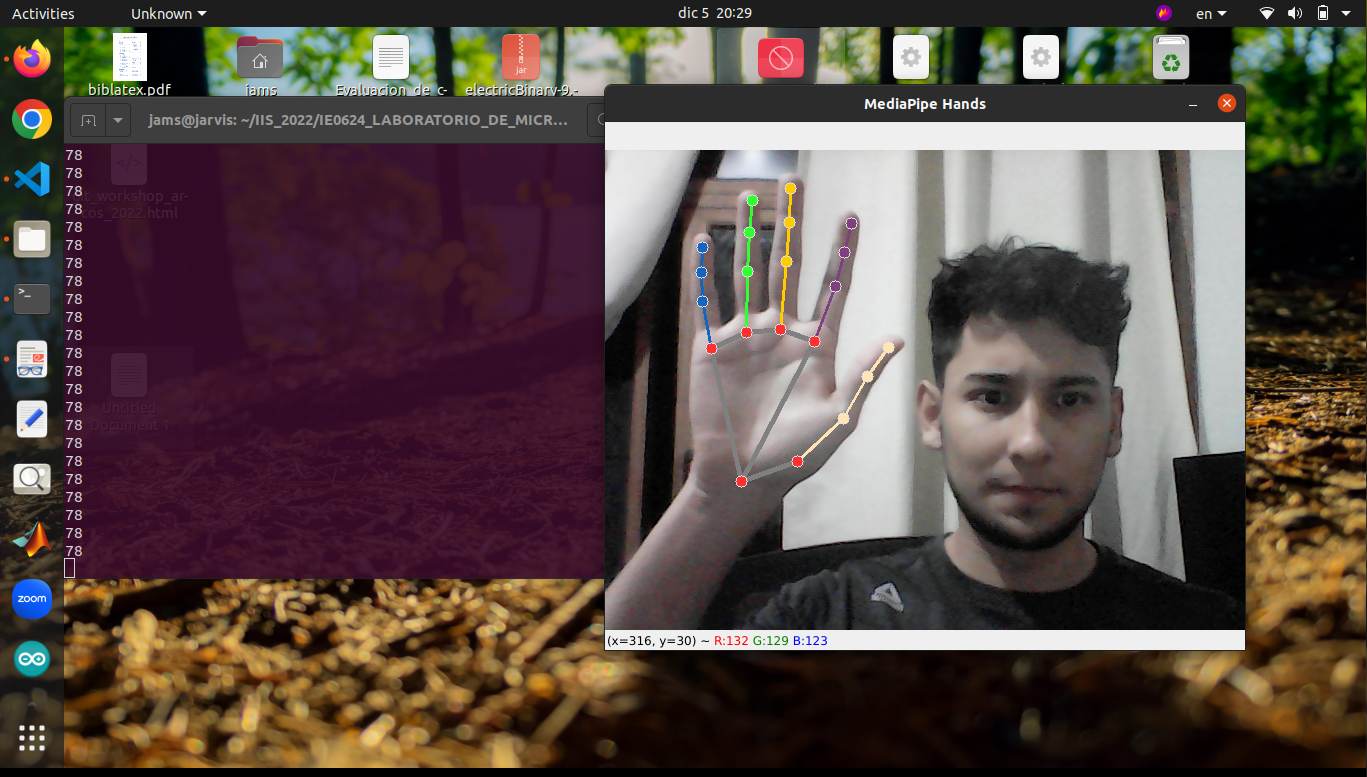
\includegraphics[scale=0.5]{./images/mano.png} 
\caption{Funcionalidad del script \texttt{hand\_recognizer.py} (Autoría propia).}
\label{mano}
\end{figure}

El funcionamiento de este script es acertado y no hay mucho más por analizar, pues su comprobación es simple. Registra aproximadamente 20 muestras por segundo y es un programa sólido.\\
Consiste primeramente en la integración de las librerías mencionadas anteriormente. Seguidamente se registran los parámetros deseados de la hora con en el orden \texttt{[hour, minute, second]} para posteriormente llegar al grueso del programa de visión por computador.\\
La sección que muestrea registra únicamente las coordenadas horizontales de la posición de la mano. En el entregable estas coordenadas no se imprimen, esto se implementa únicamente para verificar su funcionamiento. Seguidamente se entra a la parte de interacción serial con el arduino. Es muy importante resaltar que las muestras capturadas se envian como \texttt{string} al arduino por el anterior análsis dado en la sección del correspondiente al firmware. La comunicación serial presentó la dificultad de ser demasiada información para procesar por el arduino, pues el muestreo era mayor, con mayor cantidad de decimales, y con más precisión; dado esto, y debido a que para efectos de percepción humana en una señal analógica basta con al menos unos 10 puntos de luminosidad para cumplir con el objetivo del proyecto, se parametrizó las muestras en 10 estados. Los puntos de «posición» que tienen la capacidad de salir de la computadora hacia el arduino son 10: $[0, 10, 20, 30, 40, 50, 60, 70, 80, 90]$ La función \texttt{arduino} que es la encargada de enviar una parametrización de las muestras por el puerto serial, recibe un valor, dígase que este valor se encuentra entre 30 y 40, seguidamente ese valor se parametriza en en 30, y esta es la «señal» que se envía a través del puerto serial. Esto logró resolver el problema de las muestras excesivas y permitió evitar que el programa fuera más lento o se detuviera \textit{«crasheando»} la computadora.\\
Por último se crea la imagen que se ilustra en figura \ref{mano} para poder ver con facilidad los puntos específicos coloridos que registran la posición de la mano.